% Graphic for TeX using PGF
% Title: /home/di3go/workspace/t02-core-musa/doc/architecture/pictures/diagrams/stack.dia
% Creator: Dia v0.97.3
% CreationDate: Wed Dec 17 01:17:46 2014
% For: di3go
% \usepackage{tikz}
% The following commands are not supported in PSTricks at present
% We define them conditionally, so when they are implemented,
% this pgf file will use them.
\ifx\du\undefined
  \newlength{\du}
\fi
\setlength{\du}{15\unitlength}
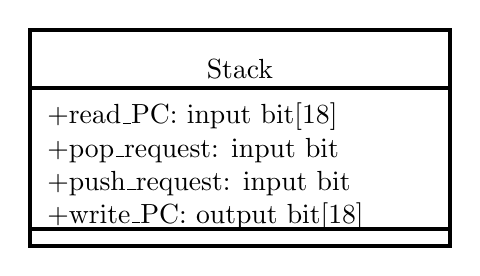
\begin{tikzpicture}
\pgftransformxscale{1.000000}
\pgftransformyscale{-1.000000}
\definecolor{dialinecolor}{rgb}{0.000000, 0.000000, 0.000000}
\pgfsetstrokecolor{dialinecolor}
\definecolor{dialinecolor}{rgb}{1.000000, 1.000000, 1.000000}
\pgfsetfillcolor{dialinecolor}
\pgfsetlinewidth{0.100000\du}
\pgfsetdash{}{0pt}
\definecolor{dialinecolor}{rgb}{1.000000, 1.000000, 1.000000}
\pgfsetfillcolor{dialinecolor}
\fill (5.100000\du,10.050000\du)--(5.100000\du,11.450000\du)--(15.225000\du,11.450000\du)--(15.225000\du,10.050000\du)--cycle;
\definecolor{dialinecolor}{rgb}{0.000000, 0.000000, 0.000000}
\pgfsetstrokecolor{dialinecolor}
\draw (5.100000\du,10.050000\du)--(5.100000\du,11.450000\du)--(15.225000\du,11.450000\du)--(15.225000\du,10.050000\du)--cycle;
% setfont left to latex
\definecolor{dialinecolor}{rgb}{0.000000, 0.000000, 0.000000}
\pgfsetstrokecolor{dialinecolor}
\node at (10.162500\du,11.000000\du){Stack};
\definecolor{dialinecolor}{rgb}{1.000000, 1.000000, 1.000000}
\pgfsetfillcolor{dialinecolor}
\fill (5.100000\du,11.450000\du)--(5.100000\du,14.850000\du)--(15.225000\du,14.850000\du)--(15.225000\du,11.450000\du)--cycle;
\definecolor{dialinecolor}{rgb}{0.000000, 0.000000, 0.000000}
\pgfsetstrokecolor{dialinecolor}
\draw (5.100000\du,11.450000\du)--(5.100000\du,14.850000\du)--(15.225000\du,14.850000\du)--(15.225000\du,11.450000\du)--cycle;
% setfont left to latex
\definecolor{dialinecolor}{rgb}{0.000000, 0.000000, 0.000000}
\pgfsetstrokecolor{dialinecolor}
\node[anchor=west] at (5.250000\du,12.150000\du){+read\_PC: input bit\ensuremath{[}18\ensuremath{]}};
% setfont left to latex
\definecolor{dialinecolor}{rgb}{0.000000, 0.000000, 0.000000}
\pgfsetstrokecolor{dialinecolor}
\node[anchor=west] at (5.250000\du,12.950000\du){+pop\_request: input bit};
% setfont left to latex
\definecolor{dialinecolor}{rgb}{0.000000, 0.000000, 0.000000}
\pgfsetstrokecolor{dialinecolor}
\node[anchor=west] at (5.250000\du,13.750000\du){+push\_request: input bit};
% setfont left to latex
\definecolor{dialinecolor}{rgb}{0.000000, 0.000000, 0.000000}
\pgfsetstrokecolor{dialinecolor}
\node[anchor=west] at (5.250000\du,14.550000\du){+write\_PC: output bit\ensuremath{[}18\ensuremath{]}};
\definecolor{dialinecolor}{rgb}{1.000000, 1.000000, 1.000000}
\pgfsetfillcolor{dialinecolor}
\fill (5.100000\du,14.850000\du)--(5.100000\du,15.250000\du)--(15.225000\du,15.250000\du)--(15.225000\du,14.850000\du)--cycle;
\definecolor{dialinecolor}{rgb}{0.000000, 0.000000, 0.000000}
\pgfsetstrokecolor{dialinecolor}
\draw (5.100000\du,14.850000\du)--(5.100000\du,15.250000\du)--(15.225000\du,15.250000\du)--(15.225000\du,14.850000\du)--cycle;
\end{tikzpicture}
